% !TEX program = xelatex
\documentclass[a4paper]{article}
\usepackage[UTF8]{ctex}
\setCJKmainfont{SimSun}[BoldFont=SimHei,ItalicFont=KaiTi]
\usepackage[top=3.2mm,bottom=3.2mm,left=3.5mm,right=3.5mm]{geometry}
\usepackage{amsmath,amssymb,bm}
\usepackage{multicol}
\usepackage{tikz}
\usetikzlibrary{arrows.meta}
\usepackage[dvipsnames]{xcolor}
\usepackage{enumitem}
\usepackage{array,tabularx}
\pagestyle{empty}
\setlength{\parindent}{0pt}
\setlength{\parskip}{0pt}
\setlength{\columnsep}{2.5mm}
\setlength{\columnseprule}{0.12pt}
\setlength{\tabcolsep}{1.1pt}
\renewcommand{\baselinestretch}{0.77}
\setlist{nosep,leftmargin=6pt,labelsep=1pt,itemsep=0pt,topsep=0pt,parsep=0pt}

\definecolor{M}{HTML}{0D47A1}
\definecolor{Q}{HTML}{1565C0}
\definecolor{R}{HTML}{B71C1C}
\definecolor{V}{HTML}{1B5E20}
\definecolor{S}{HTML}{E65100}
\definecolor{F}{HTML}{006064}
\definecolor{C}{HTML}{6A1B9A}
\definecolor{bg}{HTML}{EEF2FF}
\definecolor{warnbg}{HTML}{FFF3E0}
\newcommand{\mother}[1]{\vspace{0.35pt}{\fontsize{6.7}{6.9}\selectfont\bfseries\color{white}\colorbox{M}{\strut\;#1\;}}\par\vspace{0.15pt}}
\newcommand{\labtag}[3]{{\fontsize{4.75}{4.95}\selectfont\bfseries\color{#1}\colorbox{#1}{\color{white}\fontsize{3.75}{3.9}\selectfont #2}\,#3}\par}
\newcommand{\real}[1]{\labtag{R}{真题}{#1}}
\newcommand{\subt}[1]{\labtag{Q}{子题}{#1}}
\newcommand{\var}[1]{\labtag{V}{变式}{#1}}
\newcommand{\iden}[1]{\labtag{C}{识别}{#1}}
\newcommand{\step}[1]{\labtag{S}{步骤}{#1}}
\newcommand{\form}[1]{\labtag{F}{公式链}{#1}}
\newcommand{\err}[1]{\labtag{R}{易错}{#1}}
\newcommand{\lookup}[1]{\labtag{C}{查表}{#1}}
\newcommand{\concept}[1]{\labtag{V}{概念}{#1}}
\newcommand{\sym}[1]{\labtag{F}{符号}{#1}}
\newcommand{\boxmini}[1]{\colorbox{warnbg}{\begin{minipage}{\dimexpr\linewidth-2\fboxsep\relax}\fontsize{4.65}{4.88}\selectfont #1\end{minipage}}\par}
\newcommand{\eq}[1]{\colorbox{bg}{$\displaystyle #1$}}
\newcommand{\eqb}[1]{\par\colorbox{bg}{\begin{minipage}{\dimexpr\linewidth-2\fboxsep\relax}\centering\fontsize{5.0}{5.3}\selectfont$\displaystyle #1$\end{minipage}}\par}
\newcommand{\kw}[1]{{\bfseries\color{S}#1}}
\newcommand{\bad}[1]{{\bfseries\color{R}#1}}
\newcommand{\pvzfig}{\begin{center}\begin{tikzpicture}[>=Latex,scale=.43,every node/.style={font=\tiny}]
\draw[fill=gray!15] (0,0) rectangle (.9,1.3);\draw[fill=gray!15] (4.25,0) rectangle (5.0,.78);
\draw[dashed] (.15,1.05)--(4.85,1.05);\draw[dashed] (.15,.42)--(4.85,.42);
\draw[thick] (.9,.34)--(2.0,.34)--(2.0,.50)--(.9,.50);
\draw[thick] (2.0,.28)--(4.25,.28)--(4.25,.58)--(2.0,.58);
\draw[->,blue] (1.05,.42)--(3.9,.42);\node at (1.28,.18){A细};\node at (3.1,.14){B粗};\node at (2.0,.75){突扩};
\draw[<->] (.45,.42)--(.45,1.05);\node[left] at (.45,.74){H};\draw[<->] (4.7,.78)--(4.7,1.05);\node[right] at (4.7,.92){h};
\end{tikzpicture}\end{center}\vspace{-4pt}}
\newcommand{\lavalfig}{\begin{center}\begin{tikzpicture}[>=Latex,scale=.43,every node/.style={font=\tiny}]
\draw[thick] (0,.65).. controls (.9,.52) and (1.1,.23)..(1.85,.23).. controls (2.65,.23) and (2.9,.62)..(4.0,.75);
\draw[thick] (0,-.65).. controls (.9,-.52) and (1.1,-.23)..(1.85,-.23).. controls (2.65,-.23) and (2.9,-.62)..(4.0,-.75);
\draw[dashed] (1.85,-.5)--(1.85,.5);\node at (1.85,-.72){喉$A^*$};\draw[->,blue] (-.25,0)--(.5,0);\node at (.18,.92){$p_0,T_0$};
\draw[->,blue] (3.3,0)--(4.15,0);\node at (3.75,.95){$p_e,p_b$};\draw[red,thick] (2.9,-.55)--(2.9,.55);\node[red] at (3.15,.68){激波?};
\end{tikzpicture}\end{center}\vspace{-4pt}}
\newcommand{\cylfig}{\begin{center}\begin{tikzpicture}[>=Latex,scale=.43,every node/.style={font=\tiny}]
\foreach \y in {-.45,0,.45}{\draw[->,blue] (-.3,\y)--(.7,\y);}
\draw[thick] (1.15,0) circle (.42);\node at (1.15,-.7){圆柱/半圆柱};
\draw[->,red] (1.15,.43) arc (90:20:.43);\node[red] at (1.92,.45){$\Gamma$};
\draw[thick] (2.55,0)--(4.0,0);\draw[thick] (2.55,0)--(4.0,.52);\draw[red,thick] (2.55,0)--(3.15,1.0);\node at (3.4,.8){斜激波};
\end{tikzpicture}\end{center}\vspace{-4pt}}
\newcommand{\platefig}{\begin{center}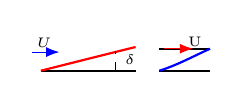
\begin{tikzpicture}[>=Latex,scale=.43,every node/.style={font=\tiny}]
\draw[thick] (0,0)--(2.8,0);\draw[->,blue] (-.25,.55)--(.55,.55);\node at (.1,.82){$U$};
\draw[red,thick] (0,0).. controls (.8,.2) and (1.9,.48)..(2.8,.7);\draw[dashed] (2.2,0)--(2.2,.58);\node[right] at (2.2,.32){$\delta$};
\draw[thick] (3.5,0)--(5.0,0);\draw[thick] (3.5,.65)--(5.0,.65);\draw[->,red] (3.65,.65)--(4.5,.65);\node at (4.55,.86){U};
\draw[blue,thick] (3.5,0).. controls (4.0,.15) and (4.55,.45)..(5.0,.65);
\end{tikzpicture}\end{center}\vspace{-4pt}}

\begin{document}
\fontsize{5.25}{5.62}\selectfont

% ===================== PAGE 1 =====================
\begin{multicols}{3}
\mother{母题1：水池/油箱/管路/泵阀/水轮机综合}
\pvzfig
\real{两油箱变径突扩管 15 分真题}
题干：两油箱液面差 $h$，钢管前段 $D_1$、后段 $D_2$，入口/出口/突扩；短管求 $Q,p_A,p_B$；长管给 $Q,L_1,L_2,e,\mu,s$ 求所需液面差。此题作为管路母题主模板。
\iden{看到什么用}
水池/油箱/大容器 + 管道 + 阀/弯头/突扩/突缩/泵/水轮机 + 求 $Q,p,H,P$。有两个自由液面：先两液面列机械能；有管内 A/B 点：再从最近液面到点列局部方程。
\subt{求流量 $Q$}
第一步写大容器液面到液面：$p=0,V=0$。若短管只局损：
\eqb{h=\sum \zeta_i\frac{V_i^2}{2g}+\frac{(V_1-V_2)^2}{2g}}
若长管：
\eqb{h=\sum \lambda_i\frac{L_i}{d_i}\frac{V_i^2}{2g}+\sum \zeta_i\frac{V_i^2}{2g}}
中间顺序：设 $Q\to A_i\to V_i=Q/A_i\to Re_i\to\lambda_i\to h_L$。
\subt{求 A/B 点压强}
先有 $Q$。A 点在细管：从上游液面到 A；B 点在粗管：从 B 到下游液面或从上游液面到 B。写：
\eqb{z_1+\frac{p_1}{\rho g}+\frac{V_1^2}{2g}=z_2+\frac{p_2}{\rho g}+\frac{V_2^2}{2g}+h_L}
最后 $p=\rho g(\text{水头})$，通常是表压。
\subt{求泵安装高度/汽蚀}
从吸水池液面到泵入口列能量；约束：
\eqb{\frac{p_{\rm in}}{\rho g}\ge \frac{p_v}{\rho g}+\Delta h_{\rm safe}}
未知安装高度就是高程差。必须用\bad{绝压}，不能用表压乱代。
\subt{求泵功率/水轮机功率}
先求扬程或水轮机水头：
\eqb{H_p=E_2-E_1+h_L,\qquad H_T=E_1-E_2-h_L}
\eqb{P_{\rm pump}=\rho gQH_p/\eta,\qquad P_T=\eta\rho gQH_T}
\subt{串联/并联管路}
串联：$Q_1=Q_2=\cdots$，总损失相加。并联：各支路两端水头损失相等，$Q=\sum Q_i$。
\form{管路公式链}
\eq{A=\pi d^2/4}, \eq{V=Q/A}, \eq{Re=Vd/\nu=\rho Vd/\mu}。层流 $\lambda=64/Re$。沿程 $h_f=\lambda(L/d)V^2/(2g)$；局部 $h_\zeta=\zeta V^2/(2g)$；突扩 $h=(V_1-V_2)^2/(2g)$。
\lookup{Moody/Colebrook}
粗糙管先算 $e/d$，再用 $Re,e/d$ 查 Moody。若题给
\eqb{\frac1{\sqrt\lambda}=-2\log_{10}\left(\frac{e/d}{3.7}+\frac{2.51}{Re\sqrt\lambda}\right)}
这是迭代式。
\err{常见扣分}
局损速度必须用局部件所在管段速度；短管才可忽略沿程；油的比重 $s$ 给出则 $\rho=s\rho_w$；汽蚀和可压缩题用绝压；泵加能、水轮机取能。

\mother{母题2：静水压/测压计/闸门/曲面/浮力}
\iden{看到什么用}
静止液体、U 管、水银、油水分层、闸门、铰链、曲面、浮体/潜体、压力中心。
\subt{U 管/多管测压计}
从已知压强端沿液柱爬：向下 $+\rho gh$，向上 $-\rho gh$，同一静止连通液体同高等压。气体柱密度小可忽略。输出前判表压/绝压/真空度。
\subt{密闭容器油水分层}
从自由面或压表所在点开始逐层加减 $\rho_i gh_i$。同一水平面若为同一种静止液体则压强相同。
\subt{平面闸门}
先形心深度 $h_c$，再合力，再压力中心：
\eqb{F=\rho gh_cA,\qquad h_D=h_c+\frac{I_G}{h_cA}}
铰链题最后对铰链取矩求拉力/支反力。
\subt{曲面压力}
水平分力等于投影面静水压力；竖直分力等于曲面上方压力体液重：
\eqb{F_H=\rho gh_{c,\text{投影}}A_{\text{投影}},\qquad F_V=\rho gV_{\text{压力体}}}
合力方向 $\tan\alpha=F_V/F_H$。
\subt{浮力/稳定}
\eq{F_B=\rho_{\text{液}}gV_{\text{排}}}。漂浮平衡：重力=浮力；判断上浮/下沉比较平均密度。稳定性用浮心、重心、定倾中心。
\err{常见扣分}
压力中心比形心深；曲面竖直分力方向看压力体位置；表压可为负，绝压不可为负；水银密度不要当水。

\mother{母题3：CV 动量，弯管/喷嘴/射流/叶片}
\iden{看到什么用}
题问“力、推力、支座反力、螺栓、法兰、喷嘴、弯管、射流冲板、叶片、转矩、功率”。
\subt{弯管/变径管受力}
先连续求 $V$，再 Bernoulli 求 $p$，最后 CV：
\eqb{\sum F_x=\dot m(V_{2x}-V_{1x}),\quad \sum F_y=\dot m(V_{2y}-V_{1y})}
压力力指向 CV 内部；求“水对管”的力，要对“管对水”的力取反。
\subt{喷嘴/消防水枪/固定板}
自由出口表压 0。若速度变大压强变小，入口压力不能漏。喷嘴反力用动量变化：入口压力 + 支反力 = 动量通量差。
\subt{射流冲击平板}
固定垂直板近似 $F=\rho QV$。斜板/分流要按 $x,y$ 分量写；若忽略损失，出口速度大小近似不变，只改方向。
\subt{运动叶片/水轮机}
绝对速度 $\bm V$，叶片速度 $\bm U$，相对速度 $\bm W=\bm V-\bm U$。功率来自切向动量变化：
\eqb{M=\dot m(r_2V_{u2}-r_1V_{u1}),\qquad P=M\omega}
\err{常见扣分}
动量方程必须用矢量分量；压力力用表压即可但全题统一；支座反力与流体受力方向相反；出口为大气压不代表速度为 0。
\end{multicols}
\newpage

% ===================== PAGE 2 =====================
\begin{multicols}{3}
\mother{母题4：势流叠加，源/汇/涡/偶极子/镜像}
\cylfig
\iden{看到什么用}
题干有“理想、不可压、无旋、势函数、流函数、圆柱绕流、壁面、镜像、点源/点汇/点涡/偶极子、Rankine体、驻点、环量、升力”。
\subt{基本流叠加}
先写 $\varphi,\psi$，总流场直接相加；再由速度公式求 $v$；最后用边界条件找常数/驻点。
\form{基本流公式表}
\renewcommand{\arraystretch}{0.74}\begin{tabular}{|p{0.20\linewidth}|p{0.34\linewidth}|p{0.34\linewidth}|}
\hline 流动 & $\varphi$ & $\psi$\\ \hline
均匀流 & $Ur\cos\theta$ & $Ur\sin\theta$\\ \hline
点源 & $\frac{Q}{2\pi}\ln r$ & $\frac{Q}{2\pi}\theta$\\ \hline
点汇 & $-\frac{Q}{2\pi}\ln r$ & $-\frac{Q}{2\pi}\theta$\\ \hline
点涡 & $\frac{\Gamma}{2\pi}\theta$ & $-\frac{\Gamma}{2\pi}\ln r$\\ \hline
偶极 & $\frac{M\cos\theta}{r}$ & $-\frac{M\sin\theta}{r}$\\ \hline
\end{tabular}\renewcommand{\arraystretch}{1}
\sym{速度关系}
直角坐标：$u=\varphi_x=\psi_y,\;v=\varphi_y=-\psi_x$。极坐标：
\eqb{v_r=\frac{\partial\varphi}{\partial r}=\frac1r\frac{\partial\psi}{\partial\theta},\quad
v_\theta=\frac1r\frac{\partial\varphi}{\partial\theta}=-\frac{\partial\psi}{\partial r}}
\subt{壁面镜像}
直壁是流线：不可穿透即 $v_n=0$。点源靠壁：同号镜像；点涡靠壁：反号镜像。解题：写真实流 + 镜像流，让壁面成为 $\psi=C$。
\subt{点源+均匀流半体}
驻点由速度为 0：$r=Q/(2\pi U)$。分界流线常用 $\psi=Q/2$。若是半平面壁面抽吸，分母常从 $2\pi$ 改成 $\pi$。
\subt{环量/流量}
沿闭曲线环量：$\Gamma=\oint \bm V\cdot d\bm l$。穿过曲线流量：$\Delta\psi$。二者不要混。
\err{常见扣分}
极坐标切向微元是 $r\,d\theta$；壁面条件是法向速度 0，不是速度全为 0；势函数多连通域可能多值；点涡除原点外无旋。

\mother{母题5：圆柱/半圆柱势流，压力积分与升力}
\real{半圆柱气膜馆 15 分真题}
半径 $a=5$m，风速 $V=10$m/s，空气密度 $\rho=1.29$，内部静压为 $p_0$。求馆外速度分布、外壁压力分布、气膜馆所受升力。
\iden{看到什么用}
圆柱/半圆柱/大风/气膜馆/无粘理论/压力分布/升力/环量。半圆柱贴地：把地面看成对称面，用完整圆柱上半部分。
\subt{无环量圆柱速度}
\eqb{v_r=V\left(1-\frac{a^2}{r^2}\right)\cos\theta,\quad
v_\theta=-V\left(1+\frac{a^2}{r^2}\right)\sin\theta}
表面 $r=a$：$v_r=0,\;v_s=2V|\sin\theta|$。
\subt{压力分布}
远处到表面用定常 Bernoulli：
\eqb{p(\theta)=p_\infty+\frac12\rho V^2(1-4\sin^2\theta),\quad C_p=1-4\sin^2\theta}
\subt{半圆柱升力}
气膜馆内部 $p_{\rm in}=p_0$，外部 $p_{\rm out}$。净压差：
\eqb{p_{\rm net}=\frac12\rho V^2(4\sin^2\theta-1)}
单位长度升力：
\eqb{F'_L=\int_0^\pi p_{\rm net}\sin\theta\,a\,d\theta=\frac53\rho V^2a}
\subt{有环量圆柱}
\eqb{v_\theta(a,\theta)=-2V\sin\theta+\frac{\Gamma}{2\pi a}}
驻点：$v_\theta=0$；升力：
\eqb{L'=\rho V\Gamma}
\concept{达朗贝尔佯谬/机翼}
无粘、无环量、前后压力对称，阻力为 0；真实阻力来自粘性边界层分离。有攻角翼型满足库塔条件后形成环量，按 $L'=\rho U\Gamma$ 产生升力。
\err{常见扣分}
压力力垂直表面，合力要投影积分；半圆柱题给的是单位长度就写 $F'$；速度越大压强越小；真实阻力不能用理想势流算。

\mother{母题6：运动学、流函数/势函数、非定常伯努利}
\subt{给速度场判不可压/无旋}
不可压：$\nabla\cdot\bm V=0$；二维 $u_x+v_y=0$。无旋：$\nabla\times\bm V=0$；二维 $\omega_z=v_x-u_y=0$。
\subt{求速度势/流函数}
若无旋，积分 $u=\varphi_x,v=\varphi_y$。若二维不可压，积分 $u=\psi_y,v=-\psi_x$。若交叉偏导不一致，说明不存在对应函数。
\subt{流线/迹线}
流线：同一时刻，$dx/u=dy/v=dz/w$。迹线：解 $dx/dt=u(x,y,z,t)$。定常流中流线与迹线重合。
\subt{U 管水柱振荡}
沿流线积分非定常 Bernoulli，速度处处相同。常见结论：
\eqb{\frac{d^2 z}{dt^2}+\frac{2g}{L}z=0,\qquad T=2\pi\sqrt{\frac{L}{2g}}}
\subt{膨胀/收缩球}
球面对称连续性：$4\pi r^2v_r=4\pi R^2\dot R$，得 $v_r=R^2\dot R/r^2$；压力用非定常伯努利。
\form{非定常无旋伯努利}
\eqb{\frac{\partial\varphi}{\partial t}+\frac{V^2}{2}+\frac{p}{\rho}+gz=C(t)}
\err{常见扣分}
不可压不等于无旋；非定常题不能删 $\partial\varphi/\partial t$；环量和流量不是一个东西；极坐标别漏 $1/r$。
\end{multicols}
\newpage

% ===================== PAGE 3 =====================
\begin{multicols}{3}
\mother{母题7：可压缩基本链，等熵、临界、质量流量}
\lavalfig
\iden{看到什么用}
Ma、声速、等熵、滞止参数、临界状态、喷管、最大流量、背压。先判：等熵段？是否跨激波？是否阻塞？
\sym{符号}
$p,T,\rho$ 为静参数；$p_0,T_0,\rho_0$ 为滞止参数；$A^*$ 是 $M=1$ 临界面积；$A_t$ 是几何喉部；$p_b$ 是外部背压；$p_e$ 是喷管出口内压。
\form{等熵 Ma 链}
\eqb{\frac{T_0}{T}=1+\frac{\gamma-1}{2}M^2}
\eqb{\frac{p_0}{p}=\left(1+\frac{\gamma-1}{2}M^2\right)^{\gamma/(\gamma-1)},\quad
\frac{\rho_0}{\rho}=\left(\frac{T_0}{T}\right)^{1/(\gamma-1)}}
空气：$T_0/T=1+0.2M^2$，$p_0/p=(1+0.2M^2)^{3.5}$。
\form{面积-马赫}
\eqb{\frac{A}{A^*}=\frac1M\left[\frac2{\gamma+1}\left(1+\frac{\gamma-1}{2}M^2\right)\right]^{\frac{\gamma+1}{2(\gamma-1)}}}
空气：
\eqb{\frac{A}{A^*}=\frac1M\left(\frac{5+M^2}{6}\right)^3}
同一个 $A/A^*>1$ 有亚声速和超声速两个根，必须按支路选。
\form{临界/最大流量}
\eqb{\frac{T^*}{T_0}=\frac2{\gamma+1}=0.833,\quad
\frac{p^*}{p_0}=\left(\frac2{\gamma+1}\right)^{\gamma/(\gamma-1)}=0.528}
\eqb{\dot m_{\max}=0.0404\,A^*p_0/\sqrt{T_0}\quad(\text{空气SI})}
\err{0.528 易错}
0.528 只属于 $M=1$ 临界状态，不是“所有喉部压力比”。喉部 $M\le1$；只有阻塞时 $A_t=A^*$、$p_t=p^*$。

\mother{母题8：Laval 喷管背压状态 + 汞柱 + 正激波}
\real{Laval 汞柱真题}
给 $p_0=300$kPa，$T_0=373$K，$A_t=10$cm$^2$，$A_e=30$cm$^2$，喉部到下游气源汞柱 $h=15$cm，左侧喉部端水银面低。求 $p_b$、是否有正激波和位置、设计工况汞柱高。
\subt{测压计反推背压}
若喉部阻塞：$p_t=p^*=0.528p_0=158.5$kPa。汞柱压差：
\eqb{\Delta p=\rho_{\rm Hg}gh=13600\times9.81\times0.15=20.0\text{kPa}}
左侧水银面低说明喉部压力更高：$p_b=p_t-\Delta p=138.5$kPa。
\subt{面积比求出口两支}
\eqb{\frac{A_e}{A_t}=3=\frac1{M_e}\left(\frac{5+M_e^2}{6}\right)^3}
解得 $M_{e,\rm sub}\approx0.197$，$M_{e,\rm sup}\approx2.637$。
\subt{三个关键背压}
亚声速支：
\eqb{p_{b1}=p_0(1+0.2M_{\rm sub}^2)^{-3.5}\approx291.95\text{kPa}}
设计超声速支：
\eqb{p_{b3}=p_0(1+0.2M_{\rm sup}^2)^{-3.5}\approx14.19\text{kPa}}
出口正激波背压：
\eqb{p_{b2}=p_{b3}\left[1+\frac{2\gamma}{\gamma+1}(M_{\rm sup}^2-1)\right]\approx112.79\text{kPa}}
\subt{判断激波位置}
若 $p_{b2}<p_b<p_{b1}$，管内有正激波；本题 $112.79<138.5<291.95$，故有正激波。因 $p_b>p_{b2}$，激波被推入喷管出口上游渐扩段。
\subt{设计工况汞柱}
设计超声速出口匹配 $p_b=p_{b3}$，喉部仍 $p_t=p^*$：
\eqb{h'=\frac{p_t-p_{b3}}{\rho_{\rm Hg}g}=\frac{158.5-14.19}{13600\times9.81}\times10^3\approx1.08\text{m}}
\err{常见扣分}
“两大气源”不是两个标准大气压；$p_b$ 是下游气源压力。跨激波后 $T_0$ 不变、$p_0$ 下降；不能用同一个 $p_0$ 从入口等熵算到全出口。

\mother{母题9：喷管其他子题，渐缩/最大流量/内激波}
\subt{渐缩喷管}
若 $p_b/p_0>0.528$：未阻塞，出口 $p_e=p_b$，由 $p_0/p_e$ 求 $M_e<1$，再算 $T,\rho,V,\dot m$。若 $p_b/p_0\le0.528$：出口临界 $M=1$，质量流量最大，继续降低背压不增流量。
\subt{给最大流量反求入口 Ma 或面积}
若给 $\dot m,A,p_0,T_0$，用质量流量函数：
\eqb{\dot m=A\frac{p_0}{\sqrt{T_0}}\sqrt{\frac{\gamma}{R}}M\left(1+\frac{\gamma-1}{2}M^2\right)^{-\frac{\gamma+1}{2(\gamma-1)}}}
若达到最大，直接 $M=1,A=A^*$。
\subt{激波在管内给定位置}
顺序：入口到激波前等熵，用 $A_s/A^*$ 求 $M_1$；过正激波求 $M_2,p_2,T_2,p_{02}$；激波后以新的 $p_{02},T_{02}$ 等熵到出口。
\lookup{查表动作}
面积-M表：输入 $A/A^*$，输出 $M$ 两支。正激波表：输入 $M_1$，输出 $M_2,p_2/p_1,T_2/T_1,p_{02}/p_{01}$。等熵表：输入 $M$，输出 $p/p_0,T/T_0,A/A^*$。
\end{multicols}
\newpage

% ===================== PAGE 4 =====================
\begin{multicols}{3}
\mother{母题10：正激波、斜激波、PM 膨胀波}
\cylfig
\iden{看到什么用}
超声速来流、波前波后绝热、压缩前后参数突变、楔形体、激波角 $\beta$、偏转角 $\theta$、Prandtl-Meyer、膨胀扇、脱体激波。
\subt{正激波}
给 $M_1,p_1,T_1$ 求波后。第一步写“波前超声，波后亚声，绝热但不可逆”。
\eqb{M_2^2=\frac{1+\frac{\gamma-1}{2}M_1^2}{\gamma M_1^2-\frac{\gamma-1}{2}}}
\eqb{\frac{p_2}{p_1}=1+\frac{2\gamma}{\gamma+1}(M_1^2-1)}
\eqb{\frac{\rho_2}{\rho_1}=\frac{(\gamma+1)M_1^2}{(\gamma-1)M_1^2+2},\qquad \frac{T_2}{T_1}=\frac{p_2/p_1}{\rho_2/\rho_1}}
\concept{正激波性质}
$M_1>1,M_2<1$；$p,T,\rho$ 上升；速度下降；$T_0$ 不变；$p_0$ 下降；熵增。
\subt{斜激波}
给 $M_1,\theta$，查 $\theta-\beta-M$ 图得弱激波 $\beta$。先法向分量：
\eqb{M_{n1}=M_1\sin\beta}
用正激波关系求 $M_{n2},p_2/p_1,T_2/T_1$，再：
\eqb{M_2=\frac{M_{n2}}{\sin(\beta-\theta)}}
切向速度不变。
\subt{PM 膨胀波}
膨胀转角 $\delta$：
\eqb{\delta=\nu(M_2)-\nu(M_1)}
空气：
\eqb{\nu(M)=\sqrt6\tan^{-1}\sqrt{\frac{M^2-1}{6}}-\tan^{-1}\sqrt{M^2-1}}
膨胀波等熵，总压不变，$M$ 增大，$p,T,\rho$ 下降。
\subt{外喷管欠/过膨胀}
若 $p_e>p_b$，出口欠膨胀，外部膨胀扇继续膨胀；若 $p_e<p_b$，过膨胀，出口外斜激波压缩；若压差大，可能激波入管或脱体。
\lookup{查表动作}
正激波表输入 $M_1$；斜激波图输入 $M_1,\theta$，输出 $\beta$；PM表输入 $M$ 输出 $\nu$，或输入 $\nu$ 反查 $M$。
\err{常见扣分}
斜激波不能直接用总 $M_1$ 套正激波，要用 $M_{n1}$；PM 是等熵，激波不是等熵；弱激波通常为物理解；转角太大没有附着斜激波，变脱体激波。

\mother{母题11：可压缩概念题归位}
\subt{阻塞为什么流量不再增大}
亚声速扰动可向上游传播，背压影响全管；喉部达到 $M=1$ 后，下游扰动不能逆传过喉部，流量由 $p_0,T_0,A^*$ 决定。
\subt{背压、出口内压、喉部压强}
$p_b$ 是外部下游环境；$p_e$ 是喷管出口截面内压；$p_t$ 是喉部静压。三者只在特定匹配状态相等。
\subt{总压为什么跨激波下降}
激波绝热但不可逆，熵增；$T_0$ 由能量守恒保持，$p_0$ 因熵增下降。
\subt{激波/膨胀波判断}
超声速气流向自己一侧压缩转弯产生斜激波；向外打开转弯产生膨胀扇。压缩升压降速，膨胀降压增速。

\mother{母题12：量纲分析与相似准则}
\iden{看到什么用}
量纲分析、$\pi$ 定理、模型试验、相似准则、阻力换算、Re/Fr/Ma 冲突。
\subt{Buckingham $\pi$ 定理}
变量 $n$ 个，基本量纲 $r$ 个，得 $n-r$ 个无量纲群。常选重复变量 $\rho,V,L$。例：阻力 $F=f(\rho,\mu,V,L)$：
\eqb{\Pi_1=\frac{F}{\rho V^2L^2},\qquad \Pi_2=\frac{\rho VL}{\mu}=Re}
故 $F=\rho V^2L^2 f(Re)$，也可写 $C_D=F/(\tfrac12\rho V^2A)$。
\subt{模型相似}
几何相似 + 运动相似 + 动力相似。常用准则：
\eqb{Re=\frac{VL}{\nu},\qquad Fr=\frac{V}{\sqrt{gL}},\qquad Ma=\frac{V}{a}}
低速外绕流看 $Re$；自由液面/船模看 $Fr$；高速可压看 $Ma$。
\subt{Re/Fr 不能同时满足}
同一流体、同一重力下，若按 $Fr$ 相似 $V\sim\sqrt L$，则 $Re\sim VL\sim L^{3/2}$，与原型不同；船模试验通常优先 Fr，阻力再修正。
\err{常见扣分}
重复变量要覆盖基本量纲且彼此独立；模型力不能只按面积比缩放，要带 $\rho V^2A$；先判断主导物理机制再选准则。

\mother{母题13：水击/水波/声速小题}
\subt{水击}
阀门迅速关闭：
\eqb{\Delta p=\rho a\Delta V,\qquad \Delta H=\frac{a\Delta V}{g}}
管壁弹性和水体压缩性会降低波速。
\subt{声速/马赫数}
\eq{a=\sqrt{\gamma RT}}，$Ma=V/a$。若飞机超声速，观察者听到声音要考虑马赫锥，$\sin\mu=1/Ma$。
\subt{线性水波}
若出现波速/波长：$\omega^2=gk\tanh kh$，深水 $\omega^2=gk$，浅水 $c=\sqrt{gh}$。只作概念入口。
\end{multicols}
\newpage

% ===================== PAGE 5 =====================
\begin{multicols}{3}
\mother{母题14：粘性精确解，N-S 简化到速度分布}
\platefig
\iden{看到什么用}
两平板、圆管、充分发展、层流、上板运动、压力梯度、剪应力、两层不混溶流体、倾斜平板、小球低 Re。
\step{通用落笔}
先写“定常、不可压、充分发展、一维”：$u=u(y)$ 或 $u=u(r)$。N-S 化为：
\eqb{0=-\frac{dp}{dx}+\mu\frac{d^2u}{dy^2}+\rho g_x}
积分两次，用边界条件定常数；剪应力 $\tau=\mu du/dy$。
\subt{普通 Couette}
下板 $u(0)=0$，上板 $u(h)=U$，无压差：$u=Uy/h$，$\tau=\mu U/h$，$q=Uh/2$。
\subt{Poiseuille 平板/圆管}
平板间压差驱动：抛物线。圆管层流：
\eqb{u(r)=u_{\max}\left(1-\frac{r^2}{R^2}\right),\quad \bar u=\frac{u_{\max}}2}
\eqb{Q=\frac{\pi R^4}{8\mu}\frac{\Delta p}{L},\quad \Delta p=\frac{32\mu VL}{d^2},\quad \lambda=64/Re}
\subt{两层 Couette}
下层 $\mu_1,h_1$，上层 $\mu_2,h_2$，上板速度 $U$。交界面速度连续、剪应力连续：
\eqb{\tau=\frac{U}{h_1/\mu_1+h_2/\mu_2}=\frac{U\mu_1\mu_2}{\mu_2h_1+\mu_1h_2}}
\eqb{u_1(y)=\frac{\tau}{\mu_1}y,\qquad u_2(y)=u_1(h_1)+\frac{\tau}{\mu_2}(y-h_1)}
\subt{倾斜平板}
沿板方向重力项 $\rho g\sin\theta$ 进入方程。若流动方向取向上：
\eqb{\mu u''+\rho g\sin\theta=0}
用 $u(0)=0,u(H)=-U_0,u(H/2)=0$ 定 $U_0$，壁面剪应力 $\tau=\mu u'$。
\subt{小球 Stokes 终速}
低 Re：
\eqb{F_D=3\pi\mu dV,\qquad V_t=\frac{(\rho_s-\rho)gd^2}{18\mu}}
算完必须回查 $Re=\rho V_td/\mu<1$。
\err{常见扣分}
两层流体相同的是剪应力，不是速度梯度；无压差不等于无重力项；层流平均速度不是最大速度；Stokes 只适合 $Re<1$。

\mother{母题15：管内层流/湍流、壁面律、摩擦系数}
\iden{看到什么用}
圆管内流动、平均速度、最大速度、管壁剪应力、线性底层、缓冲层、湍流速度分布、摩擦因数。
\subt{流态判断}
\eqb{Re=\frac{\bar u d}{\nu}}
圆管：$Re<2300$ 层流；$2300\sim4000$ 过渡；$>4000$ 湍流。题给临界值时按题给。
\subt{层流圆管}
\eqb{u(r)=2\bar u\left(1-\frac{r^2}{R^2}\right)}
\eqb{\tau_w=\frac{\Delta p\,d}{4L},\qquad \lambda=64/Re}
\subt{湍流壁面分区}
$u_*=\sqrt{\tau_w/\rho}$，$y^+=yu_*/\nu$，$u^+=u/u_*$。线性底层：$u^+=y^+$；对数区常写 $u^+=2.5\ln y^++5.5$。管内边界层厚度可用 $y^+=30$ 求 $y=30\nu/u_*$。
\subt{第1题边界层厚度类}
给 $d,\bar u,\nu$ 和提示 $\bar u/u_*=2.5\ln(Ru_*/\nu)+1.75$。流程：先由该式迭代 $u_*$；线性底层 $y^+=5$，缓冲到 $y^+=30$，完全湍流厚度约到管中心或按题给定义。
\err{常见扣分}
平均速度 $\bar u$ 不是最大速度；摩擦速度 $u_*$ 不是实际平均速度；$y^+$ 是无量纲坐标；湍流公式需自然对数还是常用对数按题给。

\mother{母题16：管路工程题与泵/水轮机}
\real{离心泵吸水管最大安装高度}
题干：吸水管粗糙、长、直径，弯头和入口阀，给流量、汽化压、大气压，要求泵入口压力至少高于汽化压某值，求泵中心高出水面的最大高度。
\subt{吸水高度}
从水面到泵入口：
\eqb{\frac{p_a}{\rho g}+z_s=\frac{p_{\rm in}}{\rho g}+z_p+\frac{V^2}{2g}+h_f+h_\zeta}
约束 $p_{\rm in}\ge p_v+\Delta p_{\rm safe}$，解 $z_p-z_s$。
\subt{水轮机输出功率}
从上游水面到下游测压点/下游水面列机械能，求水轮机水头 $H_T$，再 $P=\eta\rho gQH_T$。压力表为表压时，$p/\rho g$ 直接用表压水头。
\subt{粗糙管反推粗糙度}
已知 $Q,\Delta p,L,d$：算 $V,Re$；由能量方程反求 $\lambda$；再用 Colebrook/Moody 反推 $e/d$。
\err{常见扣分}
泵吸入口汽蚀用绝压；水轮机题高程差、压力水头、速度水头都不能漏；局部损失若题说忽略才可删。
\end{multicols}
\newpage

% ===================== PAGE 6 =====================
\begin{multicols}{3}
\mother{母题17：边界层、外绕流阻力、终端速度}
\platefig
\iden{看到什么用}
平板、边界层厚度、位移厚度、动量厚度、摩擦阻力、球/圆柱阻力、阻力系数图、终端速度。
\subt{平板层流边界层}
先 $Re_x=Ux/\nu$ 或 $Re_L=UL/\nu$。层流常用：
\eqb{\delta\approx\frac{5x}{\sqrt{Re_x}},\quad C_{f,x}=\frac{0.664}{\sqrt{Re_x}},\quad \bar C_f=\frac{1.328}{\sqrt{Re_L}}}
总摩擦阻力：$D=\bar C_f(\rho U^2/2)S$。
\subt{平板湍流/混合边界层}
湍流经验：
\eqb{\delta\approx\frac{0.37x}{Re_x^{1/5}},\qquad \bar C_f\approx\frac{0.074}{Re_L^{1/5}}-\frac{1742}{Re_L}}
混合：先算转捩点 $x_c=Re_{cr}\nu/U$，前层流后湍流，或直接用修正平均 $C_f$。
\subt{球/圆柱外绕流阻力}
\eqb{D=C_D\frac12\rho U^2A}
球 $A=\pi d^2/4$；圆柱单位长度 $A=d\times1$。$C_D$ 通常由 $Re$ 查图。
\subt{终端速度}
终速时加速度为 0：
\eqb{G-F_B-D=0}
若低 Re 用 Stokes；若一般 Re，设 $V$ 算 $Re$ 查 $C_D$，再回代，必要时迭代。
\subt{边界层概念}
位移厚度 $\delta^*=\int_0^\infty(1-u/U)dy$；动量厚度 $\theta=\int_0^\infty(u/U)(1-u/U)dy$；动量积分方程常用 $\tau_w/\rho U^2=d\theta/dx$。
\err{常见扣分}
平板用湿表面积，球/圆柱用迎风面积；局部 $C_{f,x}$ 不能当平均 $C_f$；边界层外可近似无粘，壁面附近必须有粘性。

\mother{母题18：应力张量、变形率、N-S 概念}
\iden{看到什么用}
应力张量矩阵、单位法向量、应力向量、法向/切向分量、$\nabla\cdot P$、牛顿流体、N-S 方程。
\subt{应力向量}
给 $P$ 和单位法向量 $\bm n$：
\eqb{\bm p_n=P\bm n,\quad p_{nn}=\bm p_n\cdot\bm n,\quad \bm p_t=\bm p_n-p_{nn}\bm n}
夹角：$\cos\alpha=(\bm p_n\cdot\bm n)/|\bm p_n|$。
\subt{曲面上一点应力}
先由曲面求法向量并单位化，例如 $F(x,y,z)=0$，$\bm n=\nabla F/|\nabla F|$；再代入点坐标算 $P$，最后 $P\bm n$。
\subt{散度求体力}
若给 $\rho\bm f$ 满足 $\nabla\cdot P=-\rho\bm f$，按列/行约定求散度，输出单位质量力 $\bm f$。
\concept{为什么应力张量对称}
无体偶矩时，对微元取角动量平衡，剪应力互等，所以 $P_{ij}=P_{ji}$。
\err{常见扣分}
不能直接拿矩阵某一行当应力向量；切向应力不是矩阵中的某个剪切分量，而是总应力减法向投影。

\mother{母题19：新卷快速定位总索引}
\boxmini{\kw{考试先做动作}：1圈题干关键词；2写母题编号；3写第一行主方程；4按公式链求中间量；5最后检查方向、单位、表压/绝压、查表输入、适用条件。}
\renewcommand{\arraystretch}{0.74}\begin{tabular}{|p{0.25\linewidth}|p{0.65\linewidth}|}
\hline 水池管路泵阀 & 母题1/16：PVZ，$Q\to V\to Re\to\lambda\to h_L$\\ \hline
U管闸门浮体 & 母题2：静水压链，$F=\rho gh_cA$，压力中心\\ \hline
弯管喷嘴受力 & 母题3：先能量后 CV 动量，最后取反\\ \hline
源汇涡圆柱 & 母题4/5：$\varphi,\psi$叠加，表面速度，Bernoulli 压力\\ \hline
速度场/环量 & 母题6：散度/旋度/积分，非定常保留$\varphi_t$\\ \hline
喷管/背压 & 母题7/8/9：阻塞、面积-M、背压分支、激波位置\\ \hline
斜激波/PM & 母题10：压缩斜激波，膨胀 PM，查表\\ \hline
相似/量纲 & 母题12：列变量，$\pi$ 定理，$Re/Fr/Ma$\\ \hline
平板/阻力 & 母题17：$Re_x,C_f,\delta,D$\\ \hline
应力/N-S & 母题18：$P\bm n$，N-S 简化，剪应力\\ \hline
\end{tabular}\renewcommand{\arraystretch}{1}

\mother{母题20：最终易错检查卡}
\subt{压强}
静水和管路多数用表压；汽蚀、气体、可压缩流、绝对压强题必须用绝压。$p_0$ 是滞止压，不是大气压。
\subt{方向}
CV 动量：流出-流入；支座/管壁受力与流体受力反向。压力力永远压向控制体内部。
\subt{速度}
局部损失用所在管段速度；圆管题给“平均速度”不是最大速度；叶片题分清绝对速度、相对速度、叶片速度。
\subt{状态}
喉部不是永远临界；$A_t=A^*$ 只在阻塞时成立。激波后不能继续用激波前总压。
\subt{查表}
Moody 输入 $Re,e/d$；面积-M 输入 $A/A^*$ 且选支；正激波输入 $M_1$；斜激波输入 $M_1,\theta$；PM 输入/输出 $\nu(M)$。
\subt{单位}
mm 转 m，cm$^2$ 转 m$^2$，kPa 转 Pa；汞柱 $\Delta p=\rho_{\rm Hg}gh$；比重 $s$ 转密度 $\rho=s\rho_w$。

\mother{母题21：若题目是证明/解释题}
\concept{答题骨架}
定义一句 + 适用条件一句 + 主方程一句 + 物理结论一句。不要只背结论。例：达朗贝尔佯谬=理想无粘无环量势流前后压力对称，阻力积分为零；现实阻力来自粘性分离。例：Kelvin 定理=无粘正压有势力时，封闭流体线环量守恒，所以无旋不会凭空生涡。
\concept{老师终课关键词归位}
连续介质/守恒律归母题3/6；势函数/流函数/叠加归母题4/5；激波/膨胀波/Laval归母题7-10；Re/N-S/管内压损/外绕流/边界层归母题14-17；相似准则归母题12。
\end{multicols}

\end{document}
